\documentclass[aspectratio=169,10pt]{beamer}

% ── Theme & Colors (matching Lecture 17) ────────────────────
\usetheme{metropolis}
\usepackage{appendixnumberbeamer}
\usepackage{booktabs}
\usepackage{amsmath,amssymb}
\usepackage{tikz}
\usetikzlibrary{arrows.meta,positioning,calc,decorations.pathreplacing,shapes.geometric}
\usepackage{pgfplots}
\pgfplotsset{compat=1.18}
\usepackage{xcolor}
\usepackage{graphicx}
\usepackage{multicol}

\definecolor{columbia}{RGB}{29,79,145}
\definecolor{columbialight}{RGB}{117,170,219}
\definecolor{columbiaaccent}{RGB}{210,73,42}
\definecolor{columbiagray}{RGB}{117,117,117}
\definecolor{softbg}{RGB}{245,245,250}
\definecolor{warnbg}{RGB}{255,240,230}

\setbeamercolor{frametitle}{bg=columbia,fg=white}
\setbeamercolor{progress bar}{fg=columbiaaccent}
\setbeamercolor{alerted text}{fg=columbiaaccent}
\setbeamercolor{block title}{bg=columbia,fg=white}
\setbeamercolor{block body}{bg=softbg}

\setbeamerfont{title}{size=\Large,series=\bfseries}
\setbeamerfont{frametitle}{size=\large,series=\bfseries}

\title{Health Data Modalities II:\\Modeling over EHR \& Claims Data}
\subtitle{BINF 4002 --- Machine Learning for Health \quad$\cdot$\quad Lecture 18}
\author{Matthew McDermott}
\date{March 31, 2026}
\institute{Department of Biomedical Informatics\\Columbia University}

\begin{document}
\maketitle

% ============================================================
\section{Opening}

\begin{frame}{Last Time: We Diagnosed the Problem}
\textbf{Lecture 17 established that EHR \& claims data are not ordinary ML inputs:}
\begin{itemize}[<+->]
    \item Generated as a \textbf{byproduct} of clinical care and billing --- not designed for analysis
    \item \textbf{Irregularly} timed events, not fixed feature sets or regular grids
    \item Observation is \textbf{informative} --- sicker patients generate more data
    \item \alert{Absent data $\neq$ absent condition} --- what's missing carries meaning
    \item Selection into the dataset is \textbf{structured} (Berkson's Paradox)
\end{itemize}
\begin{block}{This Lecture}
Last lecture diagnosed the pathology. This lecture asks: \emph{what does that pathology do to modeling?}
\end{block}
\end{frame}

\begin{frame}{Today's Scope: Deliberately Simple}
We will focus on \textbf{binary classification} throughout this lecture.
\vspace{0.3em}

\textbf{Why restrict ourselves?}
\begin{itemize}[<+->]
    \item So you can see what changes because of the \textbf{data modality}, not because the prediction task became mathematically exotic
    \item Binary classification is something you understand well from our ML fundamentals block
    \item Even with this ``simple'' task, the health context forces special handling
\end{itemize}
\begin{block}{Survival Models}
Survival analysis is often the principled generalization when time-to-event, censoring, and competing risks matter. There is a lab on this. Today: \emph{what issues survive even if you insist on binary classification?}
\end{block}
\end{frame}

\begin{frame}{Today's Plan}
\begin{enumerate}
    \item \textbf{Task definition:} actionability, censoring, competing risks \hfill\textcolor{columbiagray}{\scriptsize $\sim$10 min}
    \item \textbf{Three representations:} tabularized, chunked, event stream \hfill\textcolor{columbiagray}{\scriptsize $\sim$25 min}
    \item \textbf{What actually changes in the model} \hfill\textcolor{columbiagray}{\scriptsize $\sim$25 min}
    \item \textbf{Evaluation callout \& synthesis} \hfill\textcolor{columbiagray}{\scriptsize $\sim$10 min}
\end{enumerate}
\vspace{0.5em}
\begin{block}{Core Question}
If I keep the prediction objective simple --- binary classification --- what changes because the input is health event-stream data rather than ordinary ML data?
\end{block}
\end{frame}

% ============================================================
\section{Task Definition}

\begin{frame}{A Prediction Must Align with a Decision}
\textbf{``Predict X''} is incomplete unless we specify:
\begin{itemize}[<+->]
    \item \textbf{For whom?} --- Which patients are eligible (cohort)?
    \item \textbf{From when?} --- What is the prediction time / index event?
    \item \textbf{Using what?} --- What history is available at that moment?
    \item \textbf{Over what horizon?} --- What is the prediction window?
    \item \textbf{To support what action?} --- What clinical decision does this inform?
\end{itemize}
\end{frame}

\begin{frame}{Good vs.\ Bad Task Definitions}
\begin{columns}[T]
\begin{column}{0.46\textwidth}
\begin{alertblock}{Vague}
``Will this patient die?''
\begin{itemize}
    \item No prediction time
    \item No horizon
    \item No actionable decision
    \item Everyone dies eventually
\end{itemize}
\end{alertblock}
\end{column}
\begin{column}{0.50\textwidth}
\pause
\begin{exampleblock}{Actionable}
``At admission, using data available at that time, predict in-hospital mortality to guide ICU escalation.''
\begin{itemize}
    \item Clear index event
    \item Defined feature window
    \item Specific horizon
    \item Linked to a decision
\end{itemize}
\end{exampleblock}
\end{column}
\end{columns}
\vspace{0.3em}
\pause
\alert{Prediction time is part of the task definition.} A model that predicts \emph{after} the intervention window is useless even with a high AUROC.
\end{frame}

\begin{frame}{Prediction-Window Censoring}
In binary classification, we pretend every patient has a clear $\oplus$ or $\ominus$ label.
\vspace{0.3em}

\textbf{In EHR/claims, many patients are not observed long enough to know:}
\begin{itemize}[<+->]
    \item Patient transfers to another hospital
    \item Insurance coverage ends
    \item Patient simply stops seeking care
    \item Follow-up data is incomplete or delayed
\end{itemize}
\begin{alertblock}{Key Message}
\textbf{Not having an observed event $\neq$ being a true negative.}
Some of your ``negatives'' are actually \textbf{censored} --- you simply don't know what happened. If you ignore this, your model trains on corrupted labels.
\end{alertblock}
\end{frame}

\begin{frame}{Competing Risks, Even for Binary Classification}
Even if the downstream model is a binary classifier, the world contains events that make the target \textbf{impossible or change its meaning}.
\vspace{0.3em}

\textbf{Example:} Predict 30-day readmission after discharge.
\begin{itemize}[<+->]
    \item A patient who dies on day 5 cannot be readmitted
    \item A patient discharged to hospice has a fundamentally different trajectory
    \item Is a death a ``negative'' for readmission? Different from ``alive and not readmitted''
\end{itemize}
\vspace{0.2em}
Without handling this, your negative class becomes a \textbf{mixture} of: (1) true event-free patients, (2) censored patients, (3) patients for whom the event was \emph{precluded}.
\vspace{0.2em}

\alert{Competing risks are not merely a different loss function. They change what the binary label even means.}
\end{frame}

\begin{frame}{Callout: The Survival Generalization}
\begin{block}{For Reference}
\textbf{Survival models} handle these issues natively:
\begin{itemize}
    \item Time-to-event naturally accommodates censoring
    \item Competing-risk frameworks distinguish event types
    \item The prediction target becomes $P(\text{event by time } t)$, not a flat binary label
\end{itemize}
\textbf{See the survival analysis lab for hands-on practice.}
\end{block}
\vspace{0.3em}
For the rest of today: \emph{what aspects of these problems remain even if we insist on binary classification?}

\pause
Answer: nearly all of them. You still have to \textbf{define} the prediction time, handle patients whose observation ends early, and decide what to do with competing events.
\end{frame}

% ============================================================
\section{Representation Choices}

\begin{frame}{One Patient, Three Representations}
Given a patient history and a binary prediction task, we can represent the input as:
\begin{enumerate}[<+->]
    \item \textbf{Tabularized summary} --- fixed-length feature vector
    \item \textbf{Discretized temporal sequence} --- regular chunks (days, weeks, visits)
    \item \textbf{Full-resolution event stream} --- raw timestamped events
\end{enumerate}
\vspace{0.3em}
Each is defensible. Each throws away something. Each changes what ``missing'' or ``unobserved'' means.
\vspace{0.2em}
\begin{block}{Key Principle}
Most of the modeling differences in EHR are really \textbf{representation} differences.
\end{block}
\end{frame}

% ── Tabularization ──────────────────────────────────────────

\begin{frame}{Representation 1: Tabularization}
\textbf{Idea:} At each patient's \alert{prediction time}, summarize the event stream \emph{up to that point} into a fixed-length feature vector.
\vspace{0.1em}
\begin{center}
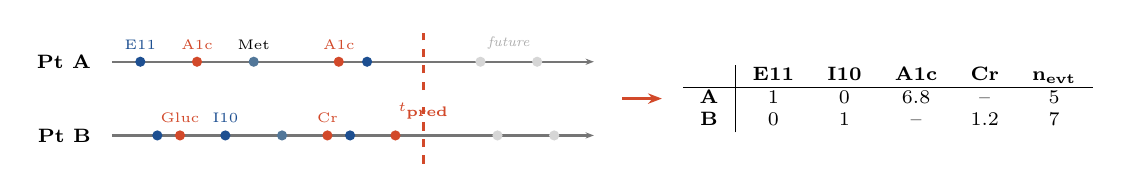
\begin{tikzpicture}[
    scale=0.72,
    evt/.style={circle, fill=columbia, inner sep=1.3pt},
    evtlab/.style={circle, fill=columbiaaccent, inner sep=1.3pt},
    evtmed/.style={circle, fill=columbialight!70!black, inner sep=1.3pt},
    futevt/.style={circle, fill=columbiagray!30, inner sep=1.3pt},
]
    % Patient A
    \node[font=\scriptsize\bfseries, anchor=east] at (-0.2, 0) {Pt A};
    \draw[-{Stealth[length=3pt]}, thick, columbiagray] (0,0) -- (8.5,0);
    \node[evt] at (0.5, 0) {};  \node[above=1pt, font=\tiny\color{columbia}] at (0.5,0) {E11};
    \node[evtlab] at (1.5, 0) {}; \node[above=1pt, font=\tiny\color{columbiaaccent}] at (1.5,0) {A1c};
    \node[evtmed] at (2.5, 0) {}; \node[above=1pt, font=\tiny] at (2.5,0) {Met};
    \node[evtlab] at (4.0, 0) {}; \node[above=1pt, font=\tiny\color{columbiaaccent}] at (4.0,0) {A1c};
    \node[evt] at (4.5, 0) {};
    % prediction time
    \draw[very thick, columbiaaccent, dashed] (5.5, -0.5) -- (5.5, 0.5);
    \node[below, font=\tiny\bfseries\color{columbiaaccent}] at (5.5, -0.55) {$t_{\text{pred}}$};
    % future (grayed)
    \node[futevt] at (6.5, 0) {};
    \node[futevt] at (7.5, 0) {};
    \node[above=1pt, font=\tiny\color{columbiagray!60}] at (7.0, 0) {\itshape future};

    % Patient B
    \node[font=\scriptsize\bfseries, anchor=east] at (-0.2, -1.3) {Pt B};
    \draw[-{Stealth[length=3pt]}, thick, columbiagray] (0,-1.3) -- (8.5,-1.3);
    \node[evt] at (0.8, -1.3) {};
    \node[evtlab] at (1.2, -1.3) {};  \node[above=1pt, font=\tiny\color{columbiaaccent}] at (1.2,-1.3) {Gluc};
    \node[evt] at (2.0, -1.3) {};  \node[above=1pt, font=\tiny\color{columbia}] at (2.0,-1.3) {I10};
    \node[evtmed] at (3.0, -1.3) {};
    \node[evtlab] at (3.8, -1.3) {}; \node[above=1pt, font=\tiny\color{columbiaaccent}] at (3.8,-1.3) {Cr};
    \node[evt] at (4.2, -1.3) {};
    \node[evtlab] at (5.0, -1.3) {};
    % prediction time
    \draw[very thick, columbiaaccent, dashed] (5.5, -1.8) -- (5.5, -0.8);
    % future (grayed)
    \node[futevt] at (6.8, -1.3) {};
    \node[futevt] at (7.8, -1.3) {};

    % Arrow to table
    \draw[-{Stealth[length=5pt]}, very thick, columbiaaccent] (9.0, -0.65) -- (9.7, -0.65);

    % Table - slightly larger font
    \node[font=\scriptsize, anchor=west] at (9.9, -0.65) {
    \begin{tabular}{c|ccccc}
    & \textbf{E11} & \textbf{I10} & \textbf{A1c} & \textbf{Cr} & \textbf{n$_\text{evt}$} \\
    \hline
    \textbf{A} & 1 & 0 & 6.8 & -- & 5 \\
    \textbf{B} & 0 & 1 & -- & 1.2 & 7 \\
    \end{tabular}
    };
\end{tikzpicture}
\end{center}
\vspace{0.1em}
\alert{Critical:} You only use data \emph{up to} the prediction time. In retrospective data, future events exist in the dataset --- using them is \textbf{label leakage}.

\pause
\vspace{0.1em}
\textbf{Requires choices at every step:} lookback window, aggregation (counts? last value?), code granularity, recency weighting\ldots
\end{frame}

\begin{frame}{Tabularization Is a Modeling Decision}
\begin{alertblock}{Not Just Preprocessing}
Tabularization is not a neutral data preparation step. It is a \textbf{large, consequential modeling decision} that can dominate the final result.
\end{alertblock}
\vspace{0.2em}
\textbf{EHR tabularized features are uniquely problematic:}
\begin{itemize}[<+->]
    \item \textbf{Highly sparse:} Most patients have a tiny fraction of possible codes
    \item \textbf{Strongly dependent:} Codes co-occur through workflow, not just biology (a blood panel produces 20+ results simultaneously)
    \item \textbf{Encode the care process:} Feature counts may reflect measurement behavior as much as underlying physiology
    \item \textbf{Ontology-sensitive:} Rolling up codes to chapter level vs.\ full detail changes which patterns are visible
\end{itemize}

\vspace{0.2em}
{\small\textbf{Optional exercise:} The ML4H MEDS Tabularization Tutorial demonstrates this.
\texttt{\color{columbia}github.com/Medical-Event-Data-Standard/MEDS\_ML4H\_2025\_Tutorial}}
\end{frame}

\begin{frame}{What ``Unobserved'' Means Under Tabularization}
Recall from last lecture: \emph{in health data, not being observed is itself informative.}
\vspace{0.2em}

Under tabularization, this creates ambiguity in every zero or missing entry:
\vspace{0.2em}
\begin{center}
{\small
\begin{tabular}{lp{8.5cm}}
\toprule
\textbf{Feature value} & \textbf{Possible meanings} \\
\midrule
No diagnosis code & No disease? Not billed? Not in our system? Not captured? \\
No lab value & Not ordered? Normal so not flagged? Measured elsewhere? \\
Zero medication count & No meds? Meds from another provider? Self-pay/OTC? \\
\bottomrule
\end{tabular}
}
\end{center}
\vspace{0.2em}
\alert{Zero, missing, and truly absent are not interchangeable in health data.} The representation collapses them all into the same cell.
\end{frame}

% ── Regular Chunking ────────────────────────────────────────

\begin{frame}{Representation 2: Regular Chunks}
\textbf{Idea:} Divide the patient timeline into fixed-width bins; create a feature vector per bin.
\vspace{0.1em}
\begin{center}
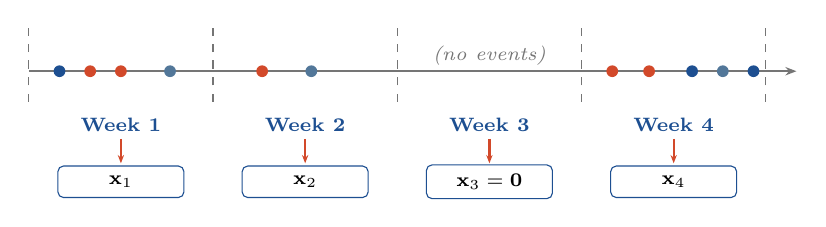
\begin{tikzpicture}[
    scale=0.78,
    evt/.style={circle, fill=columbia, inner sep=1.5pt},
    evtlab/.style={circle, fill=columbiaaccent, inner sep=1.5pt},
    evtmed/.style={circle, fill=columbialight!70!black, inner sep=1.5pt},
]
    \draw[-{Stealth[length=4pt]}, thick, columbiagray] (0,0) -- (12.5,0);
    \foreach \x in {0, 3, 6, 9, 12} {
        \draw[columbiagray, dashed] (\x,-0.5) -- (\x,0.7);
    }
    \node[below, font=\scriptsize\bfseries\color{columbia}] at (1.5, -0.6) {Week 1};
    \node[below, font=\scriptsize\bfseries\color{columbia}] at (4.5, -0.6) {Week 2};
    \node[below, font=\scriptsize\bfseries\color{columbia}] at (7.5, -0.6) {Week 3};
    \node[below, font=\scriptsize\bfseries\color{columbia}] at (10.5, -0.6) {Week 4};
    \node[evt] at (0.5, 0) {};
    \node[evtlab] at (1.0, 0) {};
    \node[evtlab] at (1.5, 0) {};
    \node[evtmed] at (2.3, 0) {};
    \node[evtlab] at (3.8, 0) {};
    \node[evtmed] at (4.6, 0) {};
    \node[font=\scriptsize\itshape\color{columbiagray}] at (7.5, 0.25) {(no events)};
    \node[evtlab] at (9.5, 0) {};
    \node[evtlab] at (10.1, 0) {};
    \node[evt] at (10.8, 0) {};
    \node[evtmed] at (11.3, 0) {};
    \node[evt] at (11.8, 0) {};
    \foreach \x in {1.5, 4.5, 7.5, 10.5} {
        \draw[-{Stealth[length=3pt]}, thick, columbiaaccent] (\x, -1.1) -- (\x, -1.5);
    }
    \node[draw=columbia, rounded corners=2pt, minimum width=1.6cm, minimum height=0.4cm, font=\scriptsize] at (1.5, -1.8) {$\mathbf{x}_1$};
    \node[draw=columbia, rounded corners=2pt, minimum width=1.6cm, minimum height=0.4cm, font=\scriptsize] at (4.5, -1.8) {$\mathbf{x}_2$};
    \node[draw=columbia, rounded corners=2pt, minimum width=1.6cm, minimum height=0.4cm, font=\scriptsize] at (7.5, -1.8) {$\mathbf{x}_3 = \mathbf{0}$};
    \node[draw=columbia, rounded corners=2pt, minimum width=1.6cm, minimum height=0.4cm, font=\scriptsize] at (10.5, -1.8) {$\mathbf{x}_4$};
\end{tikzpicture}
\end{center}
\vspace{0.1em}
\textbf{Result:} An irregularly-observed event stream becomes a \emph{regular} sequence --- compatible with RNNs, LSTMs, 1D-CNNs.

\pause
\vspace{0.2em}
\textbf{Note:} If you fix the same number of chunks for all patients (e.g., 6 one-week bins), the result is essentially a \textbf{matrix} --- a structured form of tabularization where each row is a patient and each column-group is a time window. \alert{The binning scheme is an inductive bias.}
\end{frame}

\begin{frame}{Chunking: Trade-offs and Observability}
\textbf{What it throws away:}
\begin{itemize}[<+->]
    \item Within-bin ordering disappears (lab before or after medication?)
    \item Simultaneous vs.\ same-bin events are conflated
    \item The bin width imposes a clinical timescale that may not match the task
\end{itemize}
\vspace{0.2em}
\textbf{What ``unobserved'' means here:} an empty bin is ambiguous --- healthy, not seen, data from elsewhere, or no longer enrolled.  Sparse vs.\ dense bins often encode \textbf{utilization patterns}.
\vspace{0.3em}

\textbf{The trend:} Transformer-based models increasingly operate on raw event streams, reducing the \emph{need} for chunking. But chunked representations persist for efficiency and interpretability.
\end{frame}

% ── Full Event Stream ───────────────────────────────────────

\begin{frame}{Representation 3: Full-Resolution Event Stream}
\textbf{Idea:} Keep the patient history as a sequence of timestamped events, exactly as generated.

Each event is a tuple: $(\text{time},\ \text{code},\ \text{value})$
\vspace{0.3em}

\textbf{What this preserves:}
\begin{itemize}[<+->]
    \item Fine-grained \textbf{ordering} of events
    \item Exact timing and \textbf{irregular gaps}
    \item \textbf{Repeated events} (multiple lab draws) and encounter density
\end{itemize}
\vspace{0.2em}
This is the \textbf{highest-fidelity} representation, used by the MEDS format and Lab 16.

\vspace{0.2em}
\textbf{Important:} Code granularity is a \emph{separate} design choice. You can operate on full ICD-10 codes, rolled-up categories, or any level. The event-stream format preserves temporal structure regardless of how you represent the codes within it.
\end{frame}

\begin{frame}{Event-Stream Modeling: New Burdens}
Keeping full resolution introduces design choices that don't arise otherwise:
\begin{itemize}[<+->]
    \item \textbf{Time gaps:} How to represent 6 months of silence?
    \item \textbf{Numeric values:} Lab result 7.2 is different from diagnosis E11.9. How to combine?
    \item \textbf{Simultaneous events:} An encounter can produce 50+ codes at once
    \item \textbf{Very long sequences:} ICU patients may have $>$10,000 events
    \item \textbf{Giant vocabularies:} $\sim$70,000 ICD-10 codes plus labs, meds, procedures\ldots
    \item \textbf{Sequence length $\sim$ outcome:} Sicker patients generate more events --- model can ``cheat'' by counting
\end{itemize}
\vspace{0.2em}
\textbf{What ``unobserved'' means:} No ``no-event'' tokens exist. The model must \emph{infer} from gaps and measurement patterns what absence means.
\alert{Higher-fidelity representations make care-process patterns more visible to the model, and models will exploit whatever is most predictive.} We hope coarser representations filter these out --- but they also discard genuine clinical signal.
\end{frame}

% ── Synthesis ───────────────────────────────────────────────

\begin{frame}{Comparing the Three Representations}
\vspace{-0.3em}
{\footnotesize
\begin{center}
\begin{tabular}{lp{2.6cm}p{2.6cm}p{2.6cm}}
\toprule
& \textbf{Tabularized} & \textbf{Chunked} & \textbf{Event Stream} \\
\midrule
\textbf{Preserves} & Aggregate statistics & Coarse temporal structure & Full ordering \& timing \\
\addlinespace
\textbf{Discards} & All temporal order & Within-bin order, exact timing & Nothing temporal (in principle) \\
\addlinespace
\textbf{Absence} & Zero / missing (ambiguous) & Empty bin (visible) & Long gap (must be inferred) \\
\addlinespace
\textbf{Failure mode} & Features encode care process & Bin width imposes wrong timescale & Model exploits observation density \\
\addlinespace
\textbf{Compute} & Cheapest & Moderate & Most expensive \\
\addlinespace
\textbf{Models} & Trees, logistic reg. & RNNs, 1D-CNNs & Transformers, attention \\
\bottomrule
\end{tabular}
\end{center}
}
\vspace{0.2em}
\pause
\alert{No representation is ``correct.''} The choice is a modeling decision with consequences for what your model can learn and what biases it absorbs.
\end{frame}

% ============================================================
\section{What Changes in the Model}

\begin{frame}{What Does \emph{Not} Fundamentally Change}
Before discussing what's different, what stays the same:
\begin{itemize}[<+->]
    \item You can still use \textbf{standard binary cross-entropy} loss
    \item You can still \textbf{optimize with SGD} and its variants
    \item \textbf{Train/val/test} splits still apply (with caveats)
    \item \textbf{AUROC, calibration, precision-recall} still make sense
    \item Regularization, hyperparameter tuning, ensembling --- all still apply
\end{itemize}
\begin{block}{Key Point}
Health AI is not a different discipline. The core ML machinery works. What changes is how the \textbf{input} is parameterized and what \textbf{assumptions} the data supports.
\end{block}
\end{frame}

\begin{frame}{What Changes: How to Represent Time}
In text, position 1 comes before position 2 --- simple. In EHR event streams, ``time passing'' has no single natural encoding.
\vspace{0.3em}

\textbf{Options:}
\begin{itemize}[<+->]
    \item \textbf{Absolute timestamp} (Unix time or calendar date)
    \item \textbf{Patient age} at event time
    \item \textbf{Time since previous event} (inter-event interval)
    \item \textbf{Time since last measurement of a given type}
    \item \textbf{Coarse buckets} (morning/afternoon, weekday/weekend)
    \item \textbf{Calendar features} (seasonality, day of week)
\end{itemize}
\pause
\vspace{0.2em}
Each captures a different notion of ``when.'' Combining several is common (recall Lab 16's learnable sinusoidal encodings).
\end{frame}

\begin{frame}{Time Encoding: A Counter-Intuitive Result}
\begin{alertblock}{Surprising Finding}
The marginal value of sophisticated time encodings is often \textbf{lower or more task-dependent} than expected --- and in some cases, even including explicit time tokens provides limited benefit over positional encoding alone.
\end{alertblock}
\vspace{0.2em}
\textbf{Why might this be?}
\begin{itemize}[<+->]
    \item Many signals are in the \emph{ordering} and \emph{co-occurrence} of events, not precise timing
    \item The observation process itself encodes rough timing through encounter density
    \item Contextual cues (seasonal diagnoses, age-related codes) provide implicit temporal signal
\end{itemize}
\vspace{0.2em}
% References to be added verbally: Wornow et al. (Context Clues, ICLR 2025),
% CV-Masking (NeurIPS TS4H 2025), Guo et al. (Tokenization Tradeoffs, 2026)
This ambiguity is itself a distinctive modeling issue in health event streams --- and an active research area.
\end{frame}

\begin{frame}{What Changes: Code Embeddings $\neq$ Token Embeddings}
In NLP, tokens are (mostly) arbitrary symbols. Medical codes are \textbf{structured objects}:
\begin{itemize}[<+->]
    \item \textbf{Ontology hierarchy:} \texttt{E11.65} $\subset$ \texttt{E11} (T2DM) $\subset$ Chapter IV (Endocrine)
    \item \textbf{Text descriptions:} Every code has a human-readable name
    \item \textbf{Cross-vocabulary mappings:} ICD $\leftrightarrow$ SNOMED $\leftrightarrow$ OMOP
    \item \textbf{Co-occurrence structure:} Codes that appear together in workflows
\end{itemize}
\pause
\vspace{0.2em}
\textbf{Embedding strategies that leverage this:}
\begin{itemize}
    \item \textbf{MiME} (Choi et al., NeurIPS 2018): Multilevel embeddings from visit structure
    \item \textbf{DescEmb / GenHPF} (Hur et al., 2022): Embed code \emph{text descriptions} via LMs --- enables cross-site transfer without shared vocabularies
    \item \textbf{MedTok} (2025): Multimodal tokenizer integrating text + ontology graphs
\end{itemize}
\pause
\vspace{0.2em}
\alert{In NLP, the vocabulary is discovered from data. In health AI, it comes with pre-existing structure that can be exploited --- or ignored at your peril.}
\end{frame}

% ── Foundation Models (expanded) ────────────────────────────

\begin{frame}{EHR Foundation Models: The Autoregressive Approach}
\textbf{Core idea:} Train a transformer to predict the next event in a patient's timeline.
\vspace{0.1em}
\begin{center}
    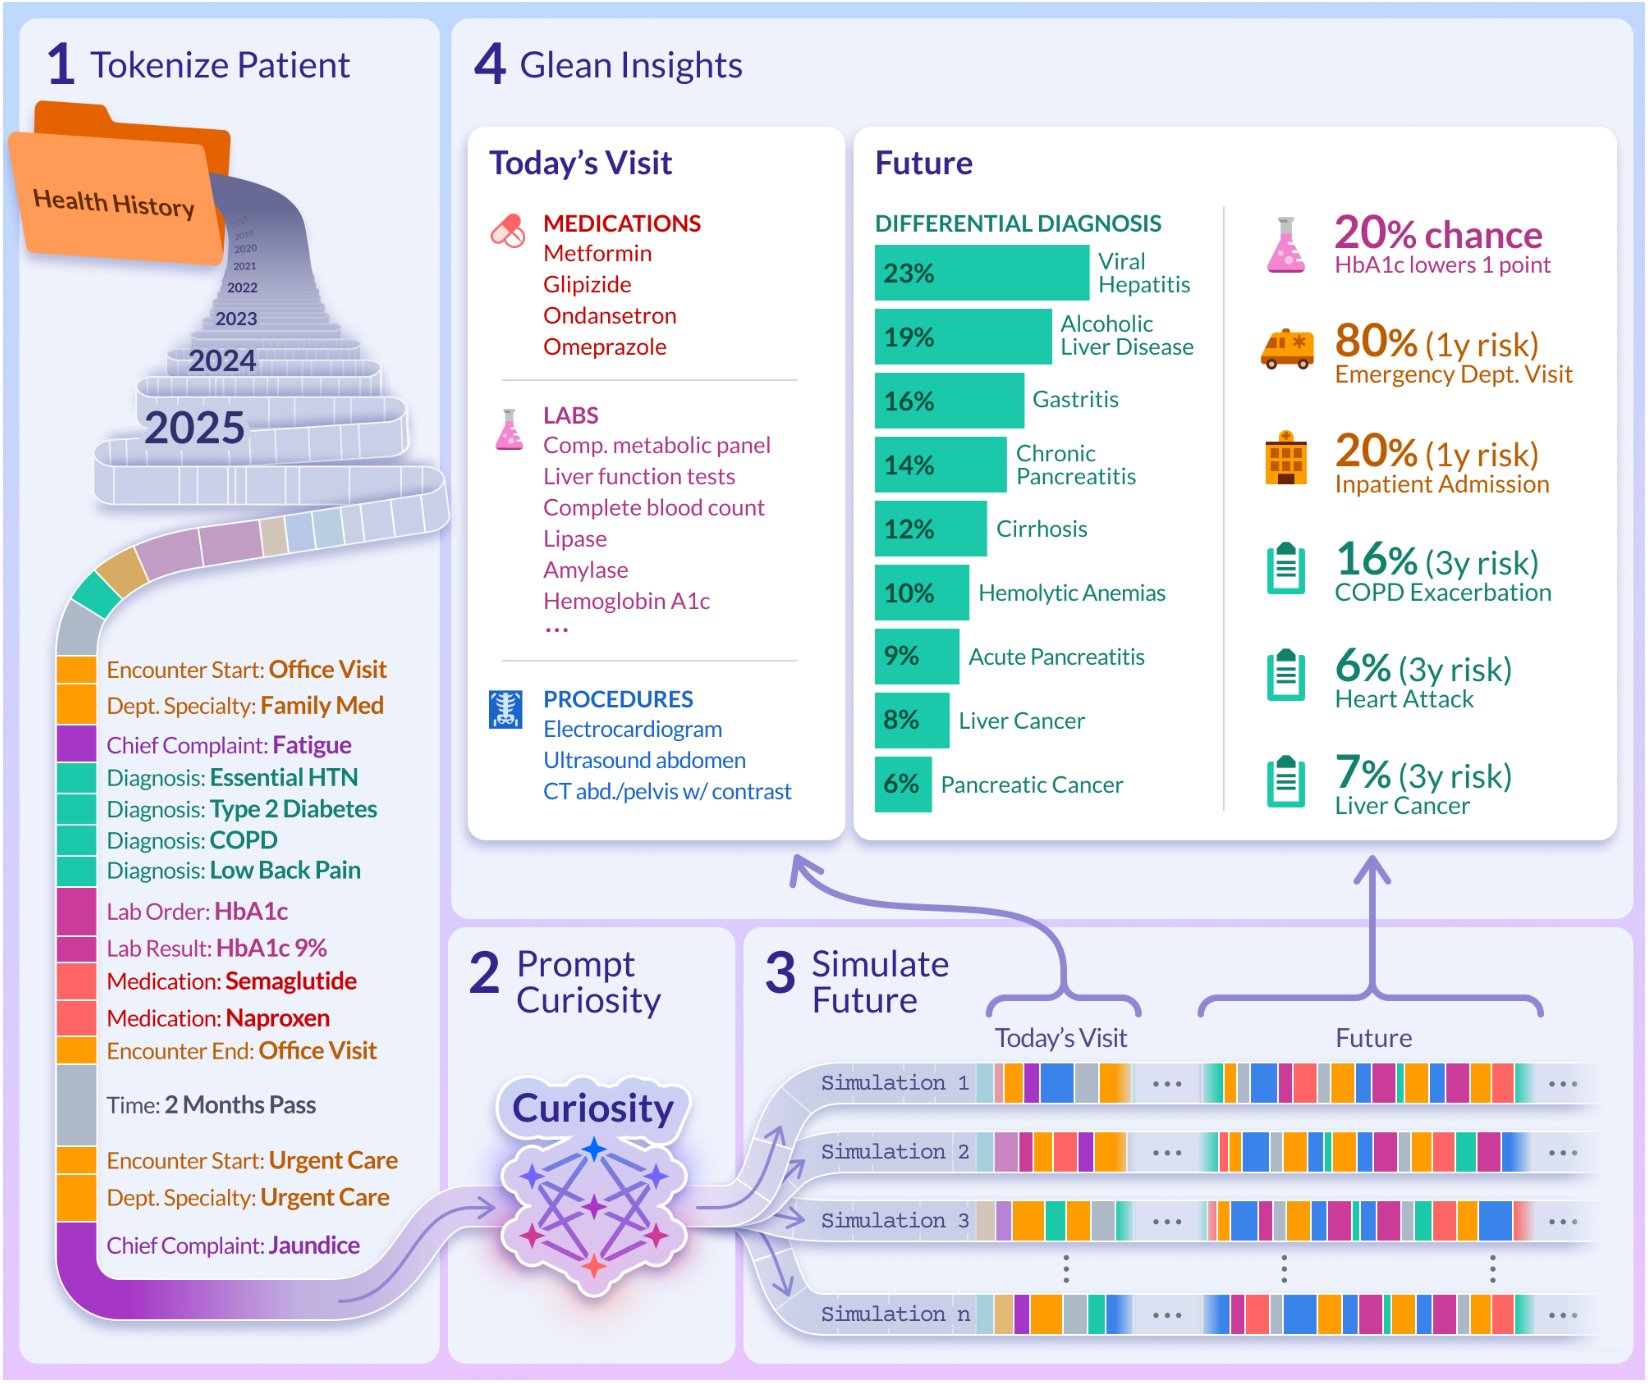
\includegraphics[height=0.55\textheight]{curiosity_figure.png}
\end{center}
\vspace{-0.2em}
{\scriptsize Figure: Curiosity pipeline (Epic; arXiv 2508.12104). 1) Tokenize history. 2) Feed to AR model. 3) \textbf{Simulate many futures.} 4) Aggregate into predictions.}
\end{frame}

\begin{frame}{How AR EHR Models Make Predictions}
Unlike an LLM, you can't just ``ask'' an EHR foundation model a question.

\vspace{0.2em}
\begin{columns}[T]
\begin{column}{0.52\textwidth}
\textbf{The inference process:}
\begin{enumerate}[<+->]
    \item Feed history up to $t_{\text{pred}}$
    \item \textbf{Autoregressively generate} many possible future trajectories
    \item Each trajectory: a sequence of future events (diagnoses, labs, meds, time gaps)
    \item \textbf{Aggregate} across simulations: ``in what fraction did event X occur within 30 days?''
\end{enumerate}
\end{column}
\begin{column}{0.46\textwidth}
\begin{center}
    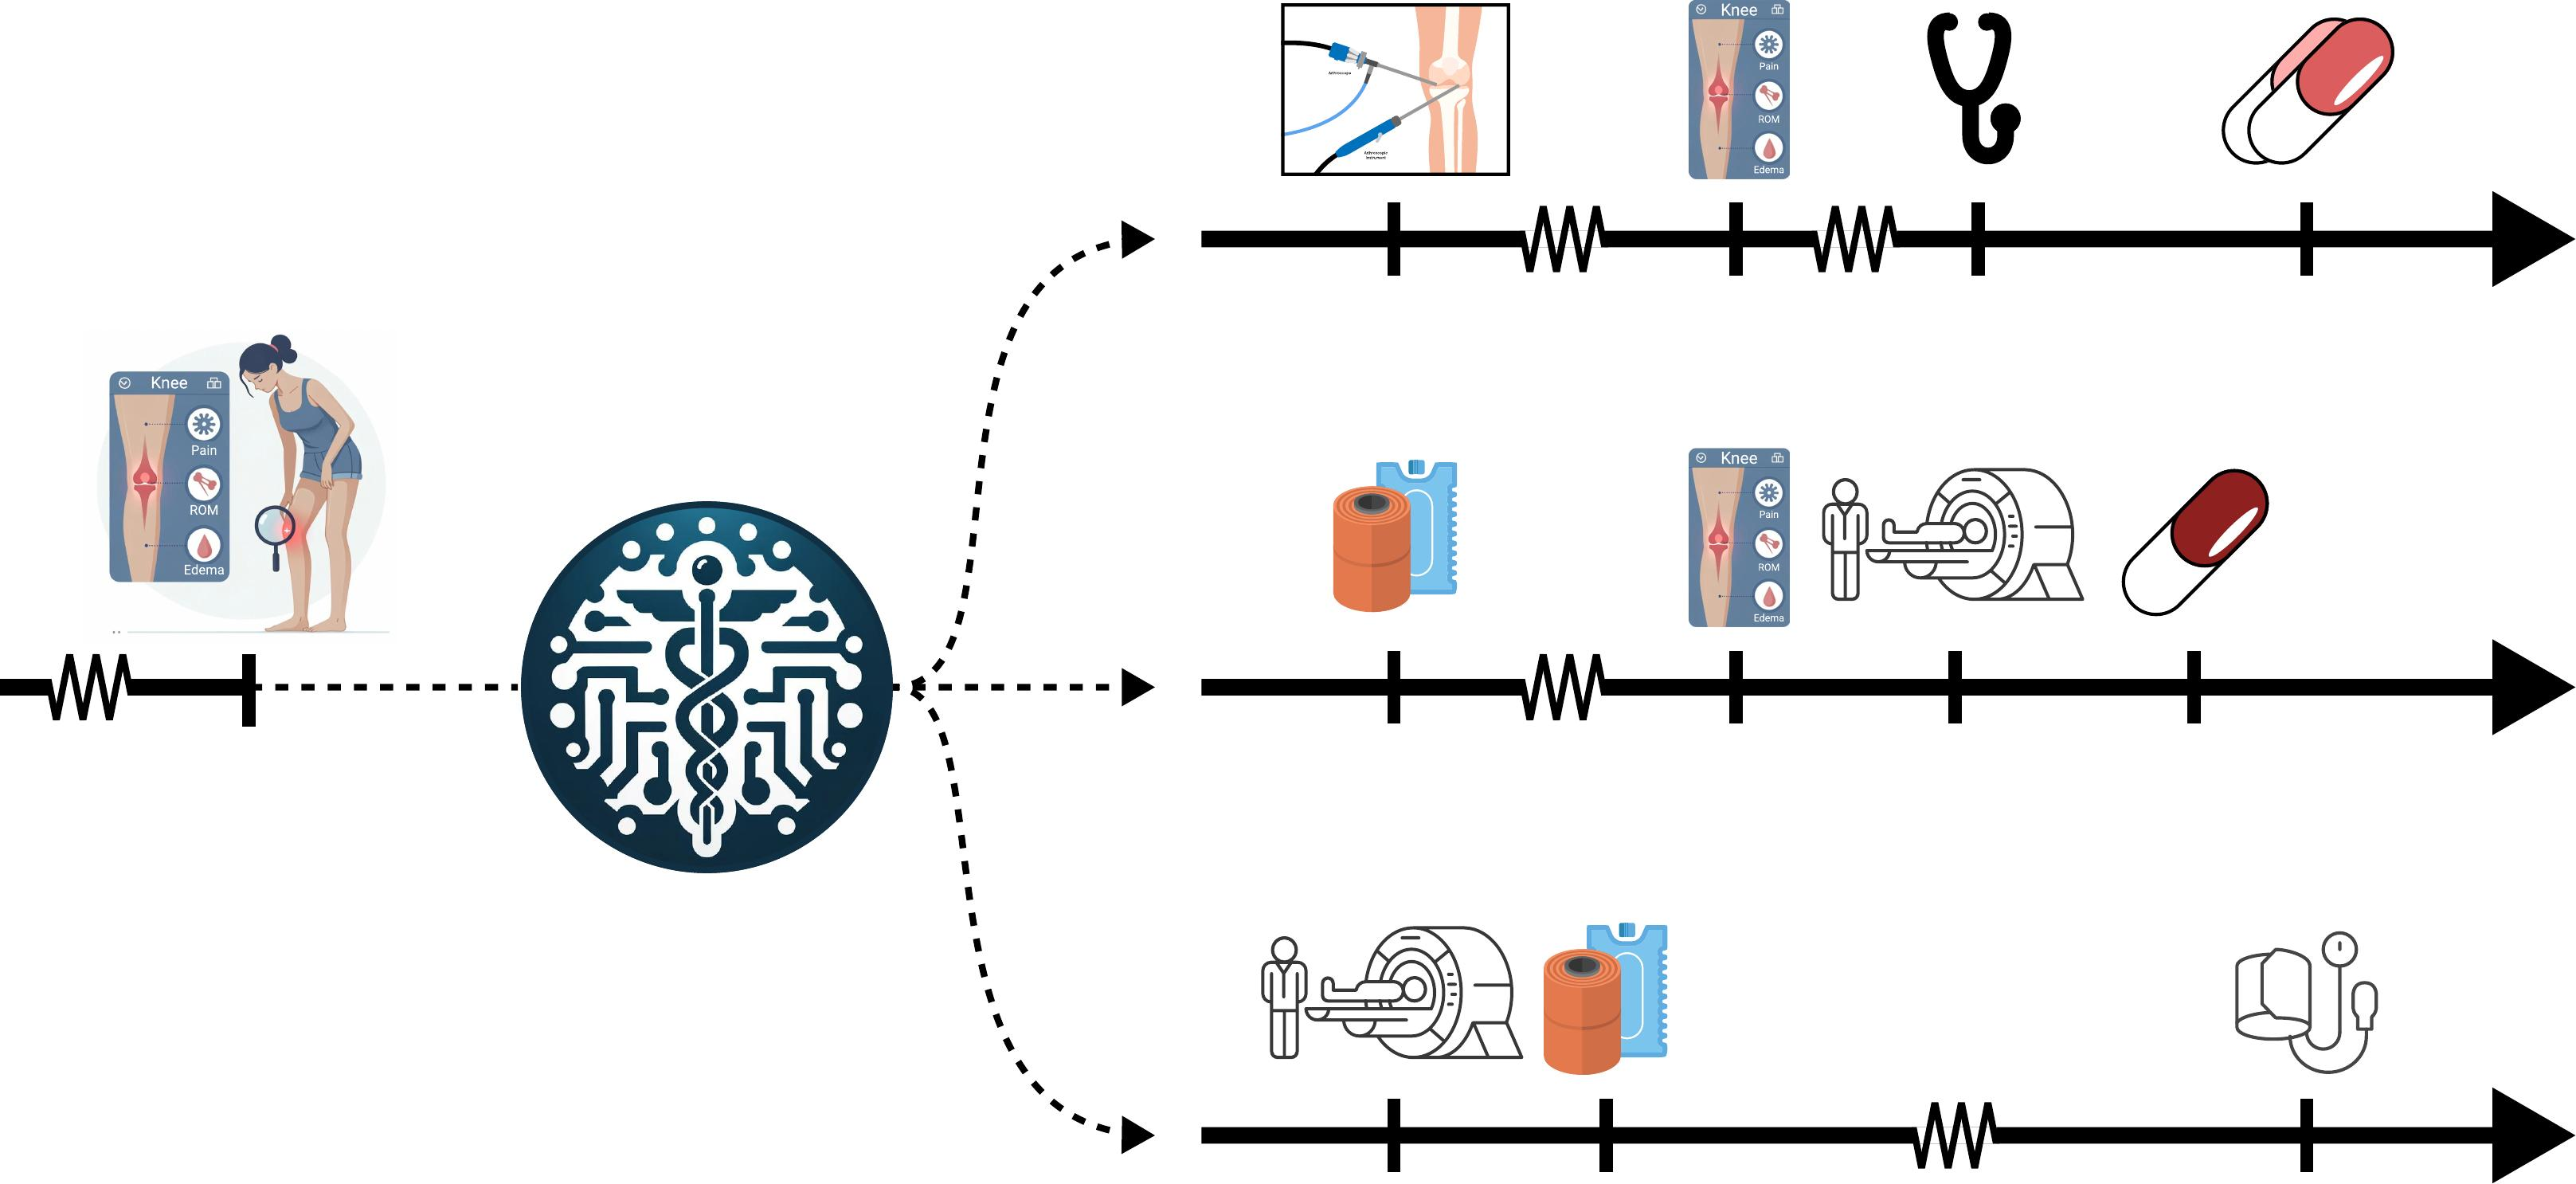
\includegraphics[width=\textwidth]{everyquery_fig.jpg}
\end{center}
\vspace{-0.3em}
{\scriptsize One patient $\to$ model $\to$ multiple sampled futures with different events and timing.}
\end{column}
\end{columns}

\vspace{0.2em}
\begin{block}{Key Point}
The model doesn't output a probability directly. It outputs \textbf{simulated futures}, and you derive probabilities by counting outcomes.
\end{block}
\end{frame}

\begin{frame}{How EHR FMs Differ from LLMs (I)}
\textbf{This is not just ``GPT but for medical codes.''} Several deep differences:

\vspace{0.3em}
\begin{enumerate}[<+->]
    \item \textbf{No prompting.} You can't ask ``will this patient develop sepsis?'' You must generate full trajectories and check. With the right prompt, an LLM needs \emph{one} forward pass for one logit. An AR EHR model needs \emph{many} generation steps $\times$ many samples.

    \item \textbf{Calibration $>$ MAP.} LLMs optimize for the most \emph{likely} continuation. EHR FMs need \emph{calibrated distributions} over futures --- the 10th percentile outcome matters as much as the mode.
\end{enumerate}
\end{frame}

\begin{frame}{How EHR FMs Differ from LLMs (II)}
\begin{enumerate}
    \setcounter{enumi}{2}
    \item<+-> \textbf{Competing generation scales.} Tokens and time are separate axes. Not all sampled trajectories will reach the prediction horizon within the token limit --- this creates \textbf{systematic statistical bias} toward shorter, event-dense futures.

    \item<+-> \textbf{Error compounding.} Because we must generate many steps to answer \emph{any} question (no single-logit shortcut), errors compound through the autoregressive chain much more than in prompted LLMs. Every additional generated token is another chance for the model to drift.
\end{enumerate}

\vspace{0.3em}
\begin{block}{The Upshot}
AR EHR FMs are maximally \emph{flexible} (any question can in principle be answered from simulated futures) but pay for that flexibility with expensive, error-prone inference.
\end{block}
\end{frame}

\begin{frame}{EveryQuery: Adding Promptability}
\textbf{EveryQuery} (Chandak et al.) takes a different approach: add ``prompting'' to EHR FMs.
\vspace{0.2em}

\textbf{The idea:}
\begin{itemize}[<+->]
    \item Instead of generating full futures and aggregating, train the model to \emph{directly answer} a specified downstream query from a single forward pass
    \item The ``query'' specifies: \emph{what} to predict, \emph{when}, over \emph{what horizon}
    \item One pre-trained model, many tasks --- without re-generating trajectories
\end{itemize}

\pause
\vspace{0.2em}
\textbf{Trade-off:}
\begin{itemize}
    \item \textbf{Gains:} Efficient inference, avoids error compounding, directly outputs calibrated probabilities
    \item \textbf{Costs:} Less flexible --- can only answer queries the model was trained to handle
\end{itemize}
\vspace{0.2em}
\alert{Broader tension:} generative EHR FMs are maximally flexible but expensive/error-prone; query-based FMs are efficient but less general.
\end{frame}

\begin{frame}{Callout: The Same Model on Claims Data}
Everything above applies to claims --- but with shifted semantics:
\vspace{0.3em}
{\small
\begin{center}
\begin{tabular}{lll}
\toprule
& \textbf{EHR} & \textbf{Claims} \\
\midrule
Time resolution & Minutes & Days--weeks \\
Generating process & Bedside care & Insurance billing \\
Observation window & Within-system & Across providers \\
Incentive bias & Documentation & Upcoding / undercoding \\
Eligibility & Visit-based & Enrollment-based \\
\bottomrule
\end{tabular}
\end{center}
}
\vspace{0.2em}
\pause
\alert{The same model may behave very differently on claims vs.\ EHR,} because the input process means something different --- even if the format looks similar.
\end{frame}

% ============================================================
\section{Evaluation \& Synthesis}

\begin{frame}{Evaluation: Don't Forget}
The representation choices from this lecture directly affect evaluation:
\begin{itemize}[<+->]
    \item Use \textbf{patient-level} splits --- never same patient in train and test
    \item Consider \textbf{time-based} splits --- train on earlier, test on later
    \item Beware \textbf{label leakage} from features recorded after the prediction time
    \item Assess \textbf{calibration} and \textbf{subgroup performance}, not just AUROC
    \item \textbf{External validation} across sites matters
\end{itemize}
\pause
\vspace{0.2em}
\textbf{Coming later:} Lectures on fairness, continuous evaluation, and deployment.
\end{frame}

\begin{frame}{Today's Takeaways}
\begin{enumerate}[<+->]
    \item \textbf{The hardest part is often not choosing a fancy model} --- it is deciding what the task and input actually are
    \item \textbf{Binary classification does not save you} from censoring, competing events, or informative observation
    \item \textbf{Representation is the main modeling lever} --- tabularized, chunked, or event stream, each with trade-offs
    \item \textbf{EHR foundation models are a fundamentally different paradigm} than LLMs --- no prompting, error compounding, competing generation scales
    \item \textbf{Modern approaches reduce the need for manual tabularization}, but do not remove the underlying clinical data problems
\end{enumerate}
\end{frame}

\begin{frame}{Looking Ahead}
\textbf{EHR is a useful middle case:} the task stays familiar, but the data-generating process forces modeling changes.
\vspace{0.5em}

\textbf{Next lectures:}
\begin{itemize}
    \item \textbf{Clinical text} --- templating, copy-paste, abbreviations, how language differs from general NLP
    \item \textbf{Medical imaging} --- where the \emph{architecture itself} changes dramatically (U-Nets, MIL)
    \item \textbf{Later:} Active learning, learning to defer, causality, fairness, continuous evaluation
\end{itemize}
\end{frame}

\begin{frame}[standout]
    Questions?
\end{frame}

% ============================================================
\appendix

\begin{frame}{Appendix: The ACES Framework for Task Definition}
\textbf{ACES} formalizes EHR prediction task definitions as machine-readable specifications:
\begin{itemize}
    \item Defines cohort selection, index events, prediction windows, label criteria
    \item Makes task definitions reproducible and shareable
    \item Separates ``what is the clinical question?'' from ``how do we extract labels?''
\end{itemize}
\vspace{0.2em}
\textbf{Key insight:} If two groups can't agree on whether a patient is positive or negative, the problem is the \emph{task definition}, not the model.

{\small\color{columbia}\texttt{github.com/justin13601/ACES}}
\end{frame}

\begin{frame}{Appendix: Phenotyping as Noisy Supervision}
A diagnosis code in the EHR is a \textbf{weak label}, not ground truth.
\begin{itemize}
    \item Billed ICD codes reflect billing incentives as much as clinical judgment
    \item Same condition coded differently across institutions / providers / time
    \item Rule-based phenotyping (e.g., eMERGE) improves specificity but adds complexity
    \item Training labels carry systematic noise correlated with features
\end{itemize}
\vspace{0.2em}
\begin{block}{Key Insight}
In many EHR prediction tasks, improving \textbf{label quality} matters more than improving model architecture.
\end{block}
\end{frame}

\begin{frame}{Appendix: Informative Observation --- A Formal View}
\textbf{Standard ML:} Features $X$ observed independently of outcome $Y$.

\textbf{EHR reality:} The observation \emph{process} depends on patient state.
\begin{itemize}
    \item $P(\text{lab ordered} \mid \text{patient state})$ is not uniform --- sicker patients get more labs
    \item $P(\text{event recorded} \mid \text{patient in system})$ depends on system factors
    \item The \textbf{number of features available} is itself a feature --- and confounded
\end{itemize}
\vspace{0.2em}
A model with access to ``how many observations does this patient have?'' can achieve nontrivial AUROC \emph{even without the content of those observations}.

\vspace{0.2em}
\textbf{Implication:} All models leverage the most predictive features available. Ask whether your representation exposes care-process patterns that dominate physiological signal.
\end{frame}

\end{document}
